\documentclass{standalone}

\usepackage{tikz}
\usepackage{tkz-euclide}

\usepackage{times}

\usetikzlibrary{positioning}
\usetikzlibrary{arrows.meta}

\definecolor{accent}{rgb}{0.9,0.9,0.9}

\begin{document}
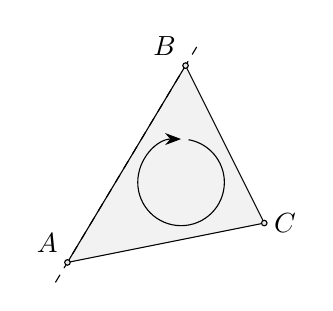
\begin{tikzpicture}[
  line/.style = {thin,dashed},
  >={Stealth[scale=1.2]},
  scale=1
]

  \tkzDefPoint(-1.0,-0.8){min}
  \tkzDefPoint(3.0,3.0){max}

  \tkzDefPoint(0,0){A}
  \tkzDefPoint(2.5,0.5){B}
  \tkzDefPoint(1.5,2.5){C}

  \tkzDrawPolygon[thin,color=black,fill=black!5](A,B,C)

  \tkzDrawSegment[line,add=0.1 and 0.1](A,C)
  % \tkzDrawSegments(A,B B,C C,A)
  \tkzDrawPoint(A)
  \tkzDrawPoint(B)
  \tkzDrawPoint(C)

  \tkzLabelPoint[right](B){$C$}
  \tkzLabelPoint[above left](C){$B$}
  \tkzLabelPoints[above left](A)

  \tkzInCenter(A,B,C)\tkzGetPoint{M}
  \tkzDefPointOnCircle[R = center M angle 90 radius 5.5mm]\tkzGetPoint{U}
  \tkzDefPointOnCircle[R = center M angle 80 radius 5.5mm]\tkzGetPoint{V}
  % \tkzDefPointOnCircle[R=]\tkzGetPoint{V}
  %\tkzDrawPoint(M)
  %\tkzDrawCircle[R](M,5.5mm)
  \tkzDrawArc[thin,color=black,<-](M,U)(V)

\end{tikzpicture}
\end{document}
